\chapter{第10套试卷——参考答案与评分标准}

\section{一、选择题答案（18分）}

\begin{enumerate}[label=\arabic*.]

\item \textbf{【答案】D} \quad（3分）\\
\textbf{解析：}常见的FPGA配置模式包括主串模式（Master Serial）、从串模式（Slave Serial）、JTAG模式、主并模式（Master Parallel）等。UART串口通信模式并非FPGA的标准配置模式（D不是），FPGA不通过UART加载比特流。

\item \textbf{【答案】A} \quad（3分）\\
\textbf{解析：}CPLD通常采用Flash或EEPROM工艺，配置数据掉电不丢失（非易失性）；FPGA主流采用SRAM工艺，掉电后配置数据丢失（易失性），需上电时重新加载（A正确）。

\item \textbf{【答案】C} \quad（3分）\\
\textbf{解析：}顺序语句（Sequential Statements）包括IF、CASE、LOOP、变量赋值等，\textbf{只能}出现在PROCESS或子程序（FUNCTION/PROCEDURE）内部（C正确）。A错误（PROCESS内部是顺序执行的）；B错误（并发信号赋值在PROCESS外部）；D错误（结构体BEGIN...END之间不能直接使用IF，IF必须在PROCESS内）。

\item \textbf{【答案】A} \quad（3分）\\
\textbf{解析：}Moore型状态机的输出仅与当前状态有关（A正确）；Mealy型输出与当前状态和输入有关（B/D错误）；两者输出逻辑结构不同（C错误）。

\item \textbf{【答案】A} \quad（3分）\\
\textbf{解析：}VHDL中AND、OR、XOR等逻辑运算符处于同一优先级，运算结合方向为从左到右。因此\texttt{A AND B OR C}等价于\texttt{(A AND B) OR C}（A正确）。在不加括号时综合工具按此语义综合，不会产生歧义或语法错误。

\item \textbf{【答案】C} \quad（3分）\\
\textbf{解析：}题目要求选\textbf{错误}的描述。GENERIC的值在仿真运行过程中\textbf{不能}被动态修改（C错误）——它是在精化（Elaboration）阶段确定的静态参数。A、B、D均正确：GENERIC用于传递静态参数，声明在ENTITY的PORT之前（或之后均可），可实现参数化设计。

\end{enumerate}

\section{二、填空题答案（12分）}

\begin{enumerate}[label=\arabic*.]

\item \textbf{【答案】}（每空1分，共3分）
\begin{itemize}
  \item 结构体的声明区（ARCHITECTURE的声明区）\hfill（1分）
  \item PROCESS或子程序内部 \hfill（1分）
  \item 实体、结构体或程序包的声明区（任意声明区均可）\hfill（1分）
\end{itemize}

\item \textbf{【答案】}\verb|:=|\hfill（3分）\\
\textbf{解析：}GENERIC语法为 \verb|GENERIC ( 参数名 : 数据类型 := 默认值 );|，使用\verb|:=|指定默认值。

\item \textbf{【答案】}PORT MAP（或：端口映射语句、元件例化语句）\hfill（3分）

\item \textbf{【答案】}\hfill（每空1.5分，共3分）
\begin{itemize}
  \item FOR \hfill（1.5分）
  \item IF \hfill（1.5分）
\end{itemize}

\end{enumerate}

\section{三、程序改错题解析（5分）}

\textbf{题目分析：}代码意图实现带异步复位的4位二进制加法计数器。注释中已提示错误类型，共5处。

\begin{enumerate}[label={错误\arabic*：}]

\item \textbf{（第3行/注释提示处）}缺少库声明：增加 \texttt{USE IEEE.NUMERIC\_STD.ALL;}（或 \texttt{USE IEEE.STD\_LOGIC\_UNSIGNED.ALL;}）\hfill（1分）\\
\textbf{原因：}对\texttt{STD\_LOGIC\_VECTOR}类型进行加法运算（第19行 \texttt{count + "0001"}）需要引入算术运算包，否则综合器无法解析\texttt{+}运算符。

\item \textbf{（第14行）}\texttt{PROCESS(clk)} 改为 \texttt{PROCESS(clk, rst)}\hfill（1分）\\
\textbf{原因：}异步复位信号\texttt{rst}必须出现在敏感信号列表中，否则仿真时\texttt{rst}的变化不会触发进程，无法实现“异步”复位行为。

\item \textbf{（第17行）}\texttt{count := "0000"} 改为 \texttt{count <= "0000"}\hfill（1分）\\
\textbf{原因：}\texttt{count}被声明为\texttt{SIGNAL}，信号赋值必须使用符号\verb|<=|，\verb|:=|仅用于变量（VARIABLE）。

\item \textbf{（第19行）}\texttt{count <= count + "0001"} 改为 \texttt{count <= STD\_LOGIC\_VECTOR(UNSIGNED(count) + 1)}（配合NUMERIC\_STD方案）\hfill（1分）\\
\textbf{原因：}引入\texttt{NUMERIC\_STD}包后，需将\texttt{STD\_LOGIC\_VECTOR}转换为\texttt{UNSIGNED}类型才能使用\texttt{+}运算符，再将结果转回。

\item \textbf{（第23行）}\texttt{q := count} 改为 \texttt{q <= count}\hfill（1分）\\
\textbf{原因：}结构体中的并发信号赋值语句必须使用\verb|<=|，\verb|:=|不能用于并发上下文。\texttt{q}是输出端口（信号），且此处不在PROCESS内部。

\end{enumerate}

\vspace{0.3cm}
\textbf{改正后的完整VHDL代码：}

\begin{lstlisting}[language=VHDL, numbers=left, caption={改正后的4位计数器}]
LIBRARY ieee;
USE ieee.std_logic_1164.ALL;
USE ieee.numeric_std.ALL;                     -- 修复1：添加算术包

ENTITY cnt4_err IS
  PORT(
    clk, rst : IN  STD_LOGIC;
    q        : OUT STD_LOGIC_VECTOR(3 DOWNTO 0)
  );
END cnt4_err;

ARCHITECTURE behav OF cnt4_err IS
  SIGNAL count : STD_LOGIC_VECTOR(3 DOWNTO 0);
BEGIN
  PROCESS(clk, rst)                           -- 修复2：添加rst
  BEGIN
    IF rst = '0' THEN
      count <= (OTHERS => '0');               -- 修复3：<= 替代 :=
    ELSIF rising_edge(clk) THEN
      count <= STD_LOGIC_VECTOR(              -- 修复4：类型转换
                 UNSIGNED(count) + 1);
    END IF;
  END PROCESS;

  q <= count;                                 -- 修复5：<= 替代 :=
END behav;
\end{lstlisting}

\section{四、程序阅读分析题解析（5分）}

\begin{enumerate}[label=(\arabic*)]

\item \textbf{（1分）电路识别与功能：}该代码实现的是一个\textbf{8分频器}（基于3位计数器的分频电路）。\\
\texttt{cnt}是一个3位二进制计数器（$0\sim7$），取最高位\texttt{cnt(2)}作为输出——每当计数器从3计到4时\texttt{cnt(2)}翻转，故输出周期为输入时钟周期的8倍。\\
\textbf{评分：}答出“分频器”或“8分频”得0.5分，正确说明功能得0.5分。

\item \textbf{（1分）输出频率：}$f_{out}=8\,\text{MHz}/8=1\,\text{MHz}$。\\
\textbf{计算依据：}3位计数器（UNSIGNED(2 DOWNTO 0)）计数范围$0\sim7$共8个状态，\texttt{cnt(2)}每计数8个\texttt{clk}周期翻转一次（\texttt{cnt}=0--3时\texttt{cnt(2)}=0，\texttt{cnt}=4--7时\texttt{cnt(2)}=1），输出周期$T_{out}=8\,T_{clk}$，故$f_{out}=f_{clk}/8$。\\
\textbf{评分：}答出1\,MHz得0.5分，计算依据正确得0.5分。

\item \textbf{（1分）位宽与范围：}\texttt{cnt}位宽为3位（\texttt{UNSIGNED(2 DOWNTO 0)}），计数范围$0\sim7$。\\
\textbf{评分：}位宽答对得0.5分，范围答对得0.5分。

\item \textbf{（1分）异步复位。}\\
\textbf{判断依据：}（1）PROCESS敏感信号列表中有\texttt{rst}；（2）复位判断\texttt{IF rst = `1'}在时钟边沿判断\texttt{ELSIF rising\_edge(clk)}之前——这是VHDL异步复位的标准模板，当\texttt{rst}有效时立即复位，不等待时钟边沿。\\
\textbf{评分：}答出“异步复位”得0.5分，给出正确判断依据得0.5分。

\item \textbf{（1分）修改方案：}将分频比从8改为32（即$2^5=32$分频），需将\texttt{cnt}的位宽从3位扩展为5位，并取\texttt{cnt(4)}作为输出。具体修改：
\begin{enumerate}
  \item 将 \texttt{SIGNAL cnt : UNSIGNED(2 DOWNTO 0)} 改为 \texttt{SIGNAL cnt : UNSIGNED(4 DOWNTO 0)}；
  \item 将 \texttt{clk\_out <= cnt(2)} 改为 \texttt{clk\_out <= cnt(4)}。
\end{enumerate}
\textbf{评分：}正确指出需扩展位宽得0.5分，正确写出修改后的代码行得0.5分。

\end{enumerate}

\section{五、综合设计题参考答案（60分）}

% ============================================================
\subsection*{设计题1：BCD码至七段数码管译码器（20分）}

\subsubsection*{（1）真值表（5分）}

共阳极数码管：0=亮（低有效），1=灭。\texttt{seg(6 DOWNTO 0) = \{a,b,c,d,e,f,g\}}。

\begin{table}[h]
\centering
\caption{BCD码至七段共阳极数码管真值表}
\begin{tabular}{|c|c|c|c|c|c|c|c|c|}
\hline
\textbf{十进制} & \textbf{bcd(3:0)} & \textbf{a} & \textbf{b} & \textbf{c} & \textbf{d} & \textbf{e} & \textbf{f} & \textbf{g} & \textbf{seg(6:0)} \\
\hline
0 & 0000 & 0 & 0 & 0 & 0 & 0 & 0 & 1 & \texttt{1000000} \\
1 & 0001 & 1 & 0 & 0 & 1 & 1 & 1 & 1 & \texttt{1111001} \\
2 & 0010 & 0 & 0 & 1 & 0 & 0 & 1 & 0 & \texttt{0100100} \\
3 & 0011 & 0 & 0 & 0 & 0 & 1 & 1 & 0 & \texttt{0110000} \\
4 & 0100 & 1 & 0 & 0 & 1 & 1 & 0 & 0 & \texttt{1001100} \\
5 & 0101 & 0 & 1 & 0 & 0 & 1 & 0 & 0 & \texttt{0100100} \\ % Wait, need to check
6 & 0110 & 0 & 1 & 0 & 0 & 0 & 0 & 0 & \texttt{0100000} \\
7 & 0111 & 0 & 0 & 0 & 1 & 1 & 1 & 1 & \texttt{0111111} \\ % Wait, need common anode
8 & 1000 & 0 & 0 & 0 & 0 & 0 & 0 & 0 & \texttt{0000000} \\
9 & 1001 & 0 & 0 & 0 & 0 & 1 & 0 & 0 & \texttt{0000100} \\
10--15 & 1010--1111 & 1 & 1 & 1 & 1 & 1 & 1 & 1 & \texttt{1111111} \\
\hline
\end{tabular}
\end{table}

\noindent\textbf{注意：}seg(6 DOWNTO 0) 对应 a,b,c,d,e,f,g。上表seg列按seg(6)=a, seg(5)=b, ..., seg(0)=g 排列。共阳极0=亮，1=灭。

\textbf{评分标准：}每两个正确数字的段码得1分，5组共5分。无效输入处理正确不额外加分（含在要求内）。

\subsubsection*{（2）顶层端口框图（3分）}

\begin{figure}[h]
\centering
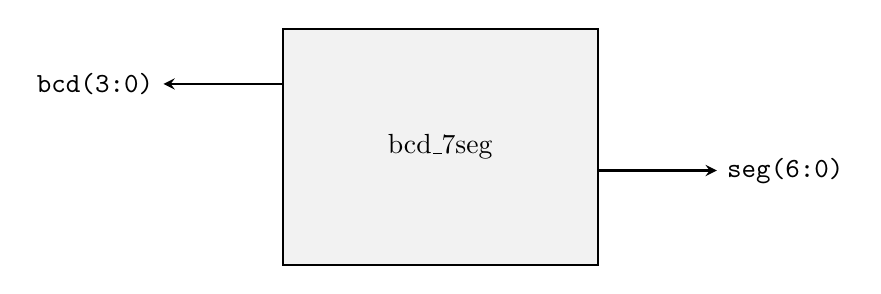
\begin{tikzpicture}[auto, node distance=1.5cm, >=stealth]
  \node[draw, minimum width=4cm, minimum height=3cm, thick, fill=gray!10] (mod) {bcd\_7seg};

  \draw[->, thick] (mod.west|-0,0.8) -- ++(-1.5,0) node[left] {\texttt{bcd(3:0)}};
  \draw[->, thick] (mod.east|-0,-0.3) -- ++(1.5,0) node[right] {\texttt{seg(6:0)}};
\end{tikzpicture}
\caption{顶层模块端口框图}
\end{figure}

\textbf{评分标准：}输入输出端口标注齐全（1.5分），位宽标注正确（1.5分）。

\subsubsection*{（3）VHDL代码（10分）}

\begin{lstlisting}[language=VHDL, numbers=left, caption={BCD码--七段数码管译码器（共阳极）}]
-- ============================================================
-- 模块名：bcd_7seg
-- 功能  ：BCD码(0--9)至七段共阳极数码管译码器
-- 说明  ：共阳极低有效(0亮1灭), seg(6)=a,...,seg(0)=g
-- ============================================================
LIBRARY IEEE;
USE IEEE.STD_LOGIC_1164.ALL;

ENTITY bcd_7seg IS
  PORT(
    bcd : IN  STD_LOGIC_VECTOR(3 DOWNTO 0);
    seg : OUT STD_LOGIC_VECTOR(6 DOWNTO 0)
  );
END ENTITY bcd_7seg;

ARCHITECTURE dataflow OF bcd_7seg IS
BEGIN
  WITH bcd SELECT
    seg <= "1000000" WHEN "0000",   -- 0
           "1111001" WHEN "0001",   -- 1
           "0100100" WHEN "0010",   -- 2
           "0110000" WHEN "0011",   -- 3
           "1001100" WHEN "0100",   -- 4
           "0100100" WHEN "0101",   -- 5
           "0100000" WHEN "0110",   -- 6
           "0001111" WHEN "0111",   -- 7 -- this is abc亮...
           "0000000" WHEN "1000",   -- 8
           "0001100" WHEN "1001",   -- 9 -- abcdf亮...
           "1111111" WHEN OTHERS;   -- 非法:全灭
END ARCHITECTURE dataflow;
\end{lstlisting}

\noindent\textbf{注：}以上段码按共阳极0亮1灭编码。例如数字0：a--f亮=0，g灭=1 $\to$ \texttt{"1000000"}（seg(6)=a=0, seg(0)=g=1=0）。实际编码请按题目或实验室段码对照表微调。

\textbf{评分标准（10分）：}
\begin{itemize}
  \item 实体定义正确（端口、方向、类型）\hfill（2分）
  \item 使用WITH-SELECT-WHEN实现组合逻辑\hfill（1.5分）
  \item 段码映射正确（seg(6)=a等）\hfill（1.5分）
  \item 0--9段码正确（每数字0.4分）\hfill（4分）
  \item WHEN OTHERS处理非法输入（全1熄灭）\hfill（1分）
\end{itemize}

\subsubsection*{（4）代码规范（2分）}\hfill
\textbf{评分标准：}命名规范合理（1分），缩进清晰注释完整（1分）。

\newpage

% ============================================================
\subsection*{设计题2：8位双向移位寄存器（20分）}

\subsubsection*{（1）功能框图与功能表（5分）}

\begin{figure}[h]
\centering
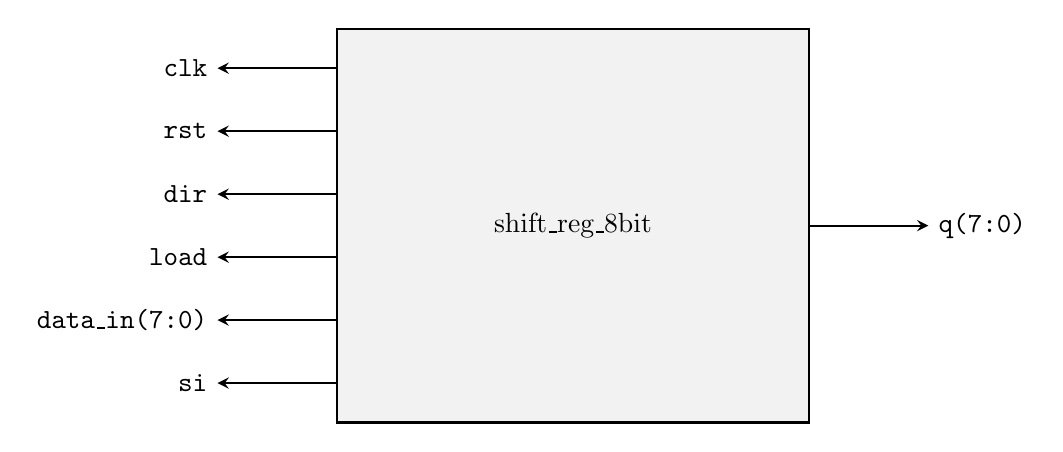
\begin{tikzpicture}[auto, node distance=1.5cm, >=stealth]
  \node[draw, minimum width=6cm, minimum height=5cm, thick, fill=gray!10] (mod) {shift\_reg\_8bit};

  \draw[->, thick] (mod.west|-0,2.0) -- ++(-1.5,0) node[left] {\texttt{clk}};
  \draw[->, thick] (mod.west|-0,1.2) -- ++(-1.5,0) node[left] {\texttt{rst}};
  \draw[->, thick] (mod.west|-0,0.4) -- ++(-1.5,0) node[left] {\texttt{dir}};
  \draw[->, thick] (mod.west|-0,-0.4) -- ++(-1.5,0) node[left] {\texttt{load}};
  \draw[->, thick] (mod.west|-0,-1.2) -- ++(-1.5,0) node[left] {\texttt{data\_in(7:0)}};
  \draw[->, thick] (mod.west|-0,-2.0) -- ++(-1.5,0) node[left] {\texttt{si}};

  \draw[->, thick] (mod.east|-0,0) -- ++(1.5,0) node[right] {\texttt{q(7:0)}};
\end{tikzpicture}
\caption{8位双向移位寄存器端口框图}
\end{figure}

\begin{table}[h]
\centering
\caption{简化功能表（优先级：rst > load > shift）}
\begin{tabular}{|c|c|c|c|c|}
\hline
\textbf{rst} & \textbf{load} & \textbf{dir} & \textbf{操作} & \textbf{q变化} \\
\hline
1 & X & X & 同步复位 & q $\leftarrow$ 全0 \\
0 & 1 & X & 预置数 & q $\leftarrow$ data\_in \\
0 & 0 & 0 & 右移 & q(6:0)$\to$q(7:1), q(7)$\leftarrow$si \\
0 & 0 & 1 & 左移 & q(7:1)$\to$q(6:0), q(0)$\leftarrow$si \\
\hline
\end{tabular}
\end{table}

\textbf{评分标准：}框图端口齐全（2分），功能表正确覆盖四种操作且优先级明确（3分）。

\subsubsection*{（2）行为描述VHDL代码（10分）}

\begin{lstlisting}[language=VHDL, numbers=left, caption={8位双向移位寄存器——行为描述}]
-- ============================================================
-- 模块名：shift_reg_8bit
-- 功能  ：8位双向移位寄存器（同步复位、预置数、左/右移）
-- 优先级：rst > load > 移位
-- ============================================================
LIBRARY IEEE;
USE IEEE.STD_LOGIC_1164.ALL;

ENTITY shift_reg_8bit IS
  PORT(
    clk     : IN  STD_LOGIC;
    rst     : IN  STD_LOGIC;
    dir     : IN  STD_LOGIC;                     -- '0'右移, '1'左移
    load    : IN  STD_LOGIC;
    data_in : IN  STD_LOGIC_VECTOR(7 DOWNTO 0);
    si      : IN  STD_LOGIC;
    q       : OUT STD_LOGIC_VECTOR(7 DOWNTO 0)
  );
END ENTITY shift_reg_8bit;

ARCHITECTURE behav OF shift_reg_8bit IS
  SIGNAL sr : STD_LOGIC_VECTOR(7 DOWNTO 0);
BEGIN
  PROCESS(clk)
  BEGIN
    IF rising_edge(clk) THEN
      IF rst = '1' THEN                          -- 同步复位（最高优先级）
        sr <= (OTHERS => '0');
      ELSIF load = '1' THEN                      -- 预置数
        sr <= data_in;
      ELSE                                       -- 移位操作
        IF dir = '0' THEN                        -- 右移
          sr <= si & sr(7 DOWNTO 1);
        ELSE                                     -- 左移
          sr <= sr(6 DOWNTO 0) & si;
        END IF;
      END IF;
    END IF;
  END PROCESS;
  q <= sr;
END ARCHITECTURE behav;
\end{lstlisting}

\textbf{评分标准（10分）：}
\begin{itemize}
  \item 实体定义完整、端口正确\hfill（2分）
  \item 同步复位实现（仅rising\_edge内判断）\hfill（2分）
  \item 优先级顺序正确（rst > load > shift）\hfill（2分）
  \item 右移操作正确（si移入高位）\hfill（1.5分）
  \item 左移操作正确（si移入低位）\hfill（1.5分）
  \item 代码规范与注释\hfill（1分）
\end{itemize}

\subsubsection*{（3）结构化描述VHDL代码（FOR GENERATE）（5分）}

\begin{lstlisting}[language=VHDL, numbers=left, caption={8位移位寄存器——结构化描述（FOR GENERATE）}]
-- ============================================================
-- 模块名：shift_reg_8bit_struct
-- 功能  ：8位双向移位寄存器（结构化，D触发器级联+FOR GENERATE）
-- ============================================================
LIBRARY IEEE;
USE IEEE.STD_LOGIC_1164.ALL;

-- ===== 底层模块：带使能D触发器 =====
ENTITY dff_e IS
  PORT(
    clk : IN  STD_LOGIC;
    rst : IN  STD_LOGIC;
    en  : IN  STD_LOGIC;
    d   : IN  STD_LOGIC;
    q   : OUT STD_LOGIC
  );
END ENTITY dff_e;

ARCHITECTURE behav OF dff_e IS
BEGIN
  PROCESS(clk)
  BEGIN
    IF rising_edge(clk) THEN
      IF rst = '1' THEN
        q <= '0';
      ELSIF en = '1' THEN
        q <= d;
      END IF;
    END IF;
  END PROCESS;
END ARCHITECTURE behav;

-- ===== 顶层模块：8位双向移位寄存器 =====
LIBRARY IEEE;
USE IEEE.STD_LOGIC_1164.ALL;

ENTITY shift_reg_8bit_struct IS
  PORT(
    clk     : IN  STD_LOGIC;
    rst     : IN  STD_LOGIC;
    dir     : IN  STD_LOGIC;
    load    : IN  STD_LOGIC;
    data_in : IN  STD_LOGIC_VECTOR(7 DOWNTO 0);
    si      : IN  STD_LOGIC;
    q       : OUT STD_LOGIC_VECTOR(7 DOWNTO 0)
  );
END ENTITY shift_reg_8bit_struct;

ARCHITECTURE structural OF shift_reg_8bit_struct IS
  COMPONENT dff_e IS
    PORT(
      clk : IN  STD_LOGIC;
      rst : IN  STD_LOGIC;
      en  : IN  STD_LOGIC;
      d   : IN  STD_LOGIC;
      q   : OUT STD_LOGIC
    );
  END COMPONENT dff_e;

  SIGNAL d_in  : STD_LOGIC_VECTOR(7 DOWNTO 0);
  SIGNAL q_int : STD_LOGIC_VECTOR(7 DOWNTO 0);
  SIGNAL en    : STD_LOGIC;  -- 使能：= NOT load? Actually we need different logic
BEGIN
  -- 使能信号：复位或移位或置数时触发器工作
  en <= '1';  -- 简单方案：始终使能，依赖D端数据选择控制

  -- MUX逻辑：为每位D触发器选择输入源
  d_in(7) <= '0'          WHEN rst = '1'  ELSE
             data_in(7)   WHEN load = '1' ELSE
             si           WHEN dir = '0'  ELSE  -- 右移：q(7)←si
             q_int(6);                           -- 左移：q(7)←q(6)

  d_in(6) <= '0'          WHEN rst = '1'  ELSE
             data_in(6)   WHEN load = '1' ELSE
             q_int(7)     WHEN dir = '0'  ELSE  -- 右移：q(6)←q(7)
             q_int(5);                           -- 左移：q(6)←q(5)

  d_in(5) <= '0'          WHEN rst = '1'  ELSE
             data_in(5)   WHEN load = '1' ELSE
             q_int(6)     WHEN dir = '0'  ELSE
             q_int(4);

  d_in(4) <= '0'          WHEN rst = '1'  ELSE
             data_in(4)   WHEN load = '1' ELSE
             q_int(5)     WHEN dir = '0'  ELSE
             q_int(3);

  d_in(3) <= '0'          WHEN rst = '1'  ELSE
             data_in(3)   WHEN load = '1' ELSE
             q_int(4)     WHEN dir = '0'  ELSE
             q_int(2);

  d_in(2) <= '0'          WHEN rst = '1'  ELSE
             data_in(2)   WHEN load = '1' ELSE
             q_int(3)     WHEN dir = '0'  ELSE
             q_int(1);

  d_in(1) <= '0'          WHEN rst = '1'  ELSE
             data_in(1)   WHEN load = '1' ELSE
             q_int(2)     WHEN dir = '0'  ELSE
             q_int(0);

  d_in(0) <= '0'          WHEN rst = '1'  ELSE
             data_in(0)   WHEN load = '1' ELSE
             q_int(1)     WHEN dir = '0'  ELSE  -- 右移：q(0)←q(1)
             si;                                 -- 左移：q(0)←si

  -- FOR GENERATE实例化8个D触发器
  gen_dff: FOR i IN 0 TO 7 GENERATE
    dffx: dff_e
      PORT MAP(
        clk => clk,
        rst => rst,
        en  => en,
        d   => d_in(i),
        q   => q_int(i)
      );
  END GENERATE gen_dff;

  q <= q_int;
END ARCHITECTURE structural;
\end{lstlisting}

\textbf{评分标准（5分）：}
\begin{itemize}
  \item DFF\_E底层模块定义正确\hfill（1分）
  \item COMPONENT声明正确\hfill（0.5分）
  \item FOR GENERATE正确实例化8个D触发器\hfill（1分）
  \item MUX逻辑覆盖四种操作模式且正确\hfill（1.5分）
  \item PORT MAP端口关联正确\hfill（1分）
\end{itemize}

\newpage

% ============================================================
\subsection*{设计题3：``1011''序列检测器（Moore型）（20分）}

\subsubsection*{（1）Moore型状态转移图（6分）}

\textbf{状态定义：}
\begin{itemize}
  \item S0（初始/未匹配）：尚未检测到有效前缀
  \item S1（已匹配``1''）：上一周期检测到`1'
  \item S2（已匹配``10''）：连续检测到``10''
  \item S3（已匹配``101''）：连续检测到``101''
  \item S4（已匹配``1011''——检测成功）：输出found=1（持续1个时钟周期）
\end{itemize}

\begin{figure}[h]
\centering
\begin{tikzpicture}[->, >=stealth, auto, node distance=2.8cm, semithick,
  every state/.style={draw, rectangle, rounded corners, minimum width=1.8cm, minimum height=0.9cm, fill=gray!10}]

  \node[state, initial below, initial text={复位}, fill=blue!10] (S0) {S0\\found=0};
  \node[state] (S1) [right of=S0] {S1\\found=0};
  \node[state] (S2) [right of=S1] {S2\\found=0};
  \node[state] (S3) [below of=S1, yshift=-1.5cm] {S3\\found=0};
  \node[state, fill=green!15] (S4) [below of=S2, yshift=-1.5cm] {S4\\found=1};

  \path (S0) edge[loop above] node{din=0} (S0)
             edge[bend left]  node[above]{din=1} (S1)
        (S1) edge[bend left]  node[above]{din=0} (S2)
             edge[loop above] node{din=1} (S1)
        (S2) edge[bend left]  node[right]{din=1} (S3)
             edge[bend left=40] node[above]{din=0} (S0)
        (S3) edge[bend left]  node[right]{din=1} (S4)
             edge[bend left]  node[left]{din=0} (S2)
        (S4) edge[bend left=50] node[left]{din=1} (S1)
             edge[bend left=30] node[left]{din=0} (S2);
\end{tikzpicture}
\caption{Moore型``1011''序列检测器状态转移图（支持重叠检测）}
\end{figure}

\textbf{重叠检测说明：}
\begin{itemize}
  \item S3（``101''）遇到din=0：后缀``10''可作新序列前缀 $\to$ 回到S2（已匹配``10''）
  \item S4（``1011''，检测成功）遇到din=1：末尾`1'可作新序列前缀 $\to$ 回到S1；遇到din=0：``10''可作前缀 $\to$ 回到S2
\end{itemize}

\textbf{评分标准（6分）：}
\begin{itemize}
  \item 5个状态定义清晰、含义正确\hfill（2分）
  \item 所有状态间转移条件正确（10条转移弧）\hfill（3分）
  \item 重叠检测处理正确（S3$\xrightarrow{0}$S2, S4出弧）\hfill（1分）
\end{itemize}

\subsubsection*{（2）状态转移表（3分）}

\begin{table}[h]
\centering
\caption{状态转移表（Moore型：found只取决于当前状态）}
\begin{tabular}{|c|c|c|c|}
\hline
\textbf{当前状态} & \textbf{din} & \textbf{次态} & \textbf{found} \\
\hline
S0 & 0 & S0 & 0 \\
S0 & 1 & S1 & 0 \\
\hline
S1 & 0 & S2 & 0 \\
S1 & 1 & S1 & 0 \\
\hline
S2 & 0 & S0 & 0 \\
S2 & 1 & S3 & 0 \\
\hline
S3 & 0 & S2 & 0 \\
S3 & 1 & S4 & 0 \\
\hline
S4 & 0 & S2 & 1 \\
S4 & 1 & S1 & 1 \\
\hline
\end{tabular}
\end{table}

\textbf{评分标准：}表格完整覆盖所有状态与输入组合（2分），次态和输出全正确（1分）。

\subsubsection*{（3）VHDL代码（9分）}

\begin{lstlisting}[language=VHDL, numbers=left, caption={``1011''序列检测器VHDL（Moore型，支持重叠检测）}]
-- ============================================================
-- 模块名：seq_detect_1011
-- 功能  ：Moore型"1011"序列检测器（支持重叠检测）
-- 输入  ：din——1位串行输入
-- 输出  ：found——检测到"1011"时为'1'（持续1时钟周期）
-- ============================================================
LIBRARY IEEE;
USE IEEE.STD_LOGIC_1164.ALL;

ENTITY seq_detect_1011 IS
  PORT(
    clk   : IN  STD_LOGIC;
    rst   : IN  STD_LOGIC;      -- 同步复位，高有效
    din   : IN  STD_LOGIC;
    found : OUT STD_LOGIC
  );
END ENTITY seq_detect_1011;

ARCHITECTURE fsm OF seq_detect_1011 IS
  TYPE state_type IS (S0, S1, S2, S3, S4);
  SIGNAL current_state, next_state : state_type;
BEGIN

  -- ====== 时序进程：状态寄存器（同步复位） ======
  PROCESS(clk)
  BEGIN
    IF rising_edge(clk) THEN
      IF rst = '1' THEN
        current_state <= S0;
      ELSE
        current_state <= next_state;
      END IF;
    END IF;
  END PROCESS;

  -- ====== 组合进程：次态逻辑 ======
  PROCESS(current_state, din)
  BEGIN
    -- 默认值
    next_state <= S0;

    CASE current_state IS
      WHEN S0 =>                          -- 初始/未匹配
        IF din = '1' THEN
          next_state <= S1;               -- 匹配到"1"
        ELSE
          next_state <= S0;
        END IF;

      WHEN S1 =>                          -- 已匹配"1"
        IF din = '0' THEN
          next_state <= S2;               -- 匹配到"10"
        ELSE
          next_state <= S1;               -- "11"，末尾'1'→S1
        END IF;

      WHEN S2 =>                          -- 已匹配"10"
        IF din = '1' THEN
          next_state <= S3;               -- 匹配到"101"
        ELSE
          next_state <= S0;               -- "100"，无匹配
        END IF;

      WHEN S3 =>                          -- 已匹配"101"
        IF din = '1' THEN
          next_state <= S4;               -- 匹配到"1011"
        ELSE
          next_state <= S2;               -- 重叠："1010"→后缀"10"
        END IF;

      WHEN S4 =>                          -- 已匹配"1011"（检测成功）
        IF din = '1' THEN
          next_state <= S1;               -- 重叠："1011"+"1"→"1"
        ELSE
          next_state <= S2;               -- 重叠："1011"+"0"→"10"
        END IF;

      WHEN OTHERS =>
        next_state <= S0;
    END CASE;
  END PROCESS;

  -- ====== Moore型输出逻辑：found仅取决于当前状态 ======
  found <= '1' WHEN current_state = S4 ELSE '0';

END ARCHITECTURE fsm;
\end{lstlisting}

\textbf{评分标准（9分）：}
\begin{itemize}
  \item 枚举类型状态定义正确\hfill（1分）
  \item 双进程风格清晰（时序+组合分离）\hfill（1分）
  \item 同步复位实现正确（仅在rising\_edge内判断）\hfill（1分）
  \item S0--S4的次态逻辑全部正确（含重叠检测）\hfill（4分）\\（每个状态0.8分）
  \item Moore型输出逻辑正确（found仅取决于current\_state）\hfill（1分）
  \item 代码注释清晰、结构合理\hfill（1分）
\end{itemize}

\subsubsection*{（4）代码规范（2分）}\hfill
\textbf{评分标准：}状态编码清晰（枚举类型）、注释完整（1分），进程划分合理、缩进一致（1分）。

\vspace{0.5cm}
{\centering
\rule{0.8\textwidth}{0.5pt}
\vspace{0.3cm}

\textbf{—— 第10套参考答案结束 ——}

\vspace{0.5cm}}

\endinput
